\documentclass[11pt,a4paper]{article}

\usepackage[margin=1in]{geometry}
\usepackage{microtype}
\usepackage{lmodern}
\usepackage[T1]{fontenc}
\usepackage[utf8]{inputenc}
\usepackage{authblk}
\usepackage{abstract}
\usepackage{booktabs}
\usepackage{listings}
\usepackage{xcolor}
\usepackage{tikz}
\usepackage{graphicx}
\graphicspath{{figures/}}
\usepackage{caption}
\usepackage{enumitem}
\usepackage{hyperref}
\usepackage{cite}
\usepackage{titlesec}

\hypersetup{
  colorlinks=true,
  linkcolor=blue!50!black,
  citecolor=blue!50!black,
  urlcolor=blue!50!black,
}

\titlespacing*{\section}{0pt}{1.2em}{0.4em}
\titlespacing*{\subsection}{0pt}{0.8em}{0.3em}

\lstdefinelanguage{yaml}{
  keywords={true,false,null,y,n},
  morestring=[b]',
  morestring=[b]",
  sensitive=false,
  comment=[l]{\#},
  morecomment=[s]{?}{:},
}
\lstset{
  basicstyle=\ttfamily\small,
  breaklines=true,
  columns=fullflexible,
  showstringspaces=false,
  keywordstyle=\color{blue!50!black}\bfseries,
  commentstyle=\color{gray}\itshape,
  stringstyle=\color{green!40!black},
  frame=single,
  framesep=4pt,
  framerule=0.4pt,
  rulecolor=\color{black!20},
  xleftmargin=4pt,
  xrightmargin=4pt,
}

\title{\vspace{-2em}\textbf{Device Context Protocol:}\\
  \large A Compact, Safety-First Architecture for\\
  LLM-Driven Control of Constrained Devices}

\author[1]{Dongxu Yang\thanks{Correspondence: \texttt{wayland0916@gmail.com}.}}
\affil[1]{deeplethe}

\date{May 2026}

\begin{document}
\maketitle

\begin{abstract}
\noindent
Large language models are increasingly used as orchestrators of external tools,
and the Model Context Protocol (MCP) has emerged as a de facto standard for
exposing such tools. MCP, however, is designed for software services running
on hosts with megabytes of memory; it does not fit on the inexpensive
microcontrollers that dominate the long tail of physical devices. Recent work
(IoT-MCP) demonstrates that an MCP server can be ported to edge gateways at a
74\,KB peak memory cost~\cite{iotmcp2025}. This still excludes the smallest,
cheapest microcontrollers, and---critically---does not address the safety
problem that arises when an unreliable caller (an LLM that may hallucinate or
be prompt-injected) is given direct control of physical hardware. We present
the \textbf{Device Context Protocol (DCP)}, a wire format and architecture
purpose-built for LLM-driven control of constrained devices. DCP composes a
6-byte header, a CBOR-encoded payload, and an optional 16-byte HMAC into a
sub-50-byte typical frame, with a reference firmware footprint targeted under
16\,KB on Cortex-M0+ class MCUs. A \emph{Bridge} process between the LLM and
the device enforces capability scoping, range and type checks, dry-run
evaluation, and units-as-types---\textbf{protocol-layer} safety primitives
that prevent malformed or hallucinated calls before any byte traverses the
device boundary. This positioning is deliberately complementary to recent
work on runtime guardrails for LLM-driven physical systems~\cite{web_of_drones,robosafe}
and post-hoc behavioral intrusion detection~\cite{aegismcp}: DCP prevents
structurally-invalid calls; those approaches catch what slips through. We
describe DCP's design rationale, MIT-licensed reference implementations
(Python Bridge, ESP32 firmware), and a language-neutral conformance suite.
We position DCP as the missing layer between MCP (which is moving toward
enterprise SaaS connectivity~\cite{mcp_roadmap_2026}) and the physical
devices it does not reach.
\end{abstract}

\section{Introduction}

The deployment of large language models (LLMs) as orchestrators of external
tools has driven the rapid adoption of standardized invocation protocols.
The Model Context Protocol (MCP)~\cite{mcp2024} has emerged as a leading
candidate, providing a JSON-RPC--based interface for exposing tools, resources,
and prompts to LLM clients such as Claude Desktop, IDE assistants, and agent
frameworks. The MCP roadmap for 2026~\cite{mcp_roadmap_2026} foregrounds
\emph{enterprise readiness}: stateless HTTP transport, OAuth~2.1,
audit logging, and gateway architectures. It says nothing about embedded
devices, and there is no indication that the upstream specification will
descend to that layer.

This produces a gap. Physical devices---smart-home actuators, sensors,
laboratory equipment, prototyping hardware---are typically built on
microcontrollers whose flash and SRAM budgets are an order of magnitude
smaller than those a JSON-RPC-over-WebSocket implementation requires. A
common workaround is to bridge the device to an MCP host with an ad-hoc
serial protocol; every project that does so reinvents framing, manifest
exchange, error reporting, and safety.

A recent academic contribution, IoT-MCP~\cite{iotmcp2025}, demonstrates that
MCP can be ported to edge devices at a 74\,KB peak memory cost and
$\sim$\,205\,ms response time across 22 sensor types and 6 microcontroller
units. We regard this as foundational empirical work that establishes the
feasibility of LLM-IoT bridging. It also surfaces three open issues: (i) the
74\,KB footprint excludes the smallest commodity MCUs (Cortex-M0+, ATmega-class,
and most BLE-only chips); (ii) the underlying protocol is unchanged MCP, so
its overhead and discovery model carry through unmodified; (iii) the paper
does not address authentication, capability scoping, or safety against
hallucinated or adversarial LLM calls---the central reliability problem
introduced by allowing an unreliable caller to control hardware.

Concurrent threat-modeling work formalizes the third concern. A recent
STRIDE-based analysis of LLM-enabled robotic systems~\cite{prompt_to_actuation}
identifies six boundary-crossing interaction points at which semantic
validation is absent in today's stacks, with no protocol-layer defenses
available to close the gap. Adjacent work proposes runtime
guardrails~\cite{web_of_drones,robosafe} and post-hoc behavioral intrusion
detection~\cite{aegismcp}, but none addresses the boundary at the
wire-format and schema level. DCP is, to our knowledge, the first proposal
to do so.

We claim that closing these issues requires changes at the protocol layer,
not the implementation layer. \textbf{DCP} (Device Context Protocol) is
our proposal: a compact wire format, a manifest schema, a safety model, and
a reference implementation across host (Python) and device (C++ for ESP32),
designed from the start for LLM callers.

\paragraph{Contributions.} This paper makes the following contributions:

\begin{enumerate}[leftmargin=*,nosep]
  \item A wire format and manifest schema (\S\ref{sec:design}) explicitly
        designed for the \emph{LLM-as-caller} setting: intent-level commands
        rather than register-level; units as a protocol primitive; dry-run as
        a wire-format bit; and a 6-byte fixed header that makes static
        dispatch on resource-constrained MCUs natural.
  \item An architectural pattern (\S\ref{sec:safety}) in which a host-side
        \emph{Bridge} is the sole trust boundary. Capability tokens
        (HMAC-SHA256, scoped, time-limited) bound the LLM's reach; range,
        type, and dry-run checks reject hallucinated calls before they
        traverse the wire. Devices remain simple.
  \item Reference implementations (\S\ref{sec:impl}): a Python Bridge with
        five transports (loopback, UART with COBS+CRC, MQTT, BLE GATT, and
        an MCP server wrapper that surfaces DCP devices to any MCP host);
        and an Arduino-compatible ESP32 firmware targeting $<\!16$\,KB
        flash, with self-contained SHA-256 for optional per-frame integrity.
  \item A language-neutral conformance suite (\S\ref{sec:impl}): a YAML
        encoding of golden frames that other implementations
        (e.g.\ in C, Rust, Go) can mechanically verify against. We argue
        this methodology is necessary for the protocol to survive
        multi-author implementation.
  \item A discussion (\S\ref{sec:related}) positioning DCP against MCP,
        IoT-MCP, W3C Web of Things~\cite{wot_td_2025},
        Matter~\cite{matter_spec}, Sparkplug~B~\cite{sparkplug}, and direct
        OpenAPI exposure. We argue DCP occupies a specific gap: \emph{LLM-native
        safety primitives at MCU scale}, which none of the alternatives
        addresses.
\end{enumerate}

We make no claim of empirical superiority on benchmarks beyond what
IoT-MCP has already reported, because we have not yet completed the
hardware measurement campaign that would justify such a claim. We position
this paper as a \emph{design contribution and architectural argument},
with a complete open-source implementation~\cite{wot_td_2025}\footnote{
The DCP reference implementation is MIT-licensed and will be released at
\texttt{github.com/device-context-protocol} upon paper acceptance.}
available for inspection and reproduction.

\section{Background: The LLM--Hardware Gap}

\subsection{Why MCP does not descend}

A minimal MCP server requires JSON parsing, a WebSocket or stdio transport,
a tool registry, and dynamic schema exchange via \texttt{tools/list}. Even
liberal implementations land near 80--120\,KB of compiled code and several
tens of kilobytes of working memory on a 32-bit MCU; IoT-MCP measured
74\,KB peak~\cite{iotmcp2025}. This excludes a large class of devices:

\begin{itemize}[leftmargin=*,nosep]
  \item Cost-driven smart-home and consumer hardware on Cortex-M0+ class MCUs
        with 32--64\,KB flash and 4--8\,KB RAM.
  \item BLE-only peripherals (e.g.\ wearables, sensors) where the BLE stack
        already consumes the majority of available memory.
  \item Battery-powered sensors that cannot afford the wake-time of a
        WebSocket handshake.
\end{itemize}

The MCP 2026 roadmap~\cite{mcp_roadmap_2026} reinforces this divergence: it
explicitly prioritizes ``production connectivity'' (statelessness, gateways,
identity) over device-scale optimization. We read this as a deliberate scope
decision and a stable boundary on which to build downstream.

\subsection{Why LLMs are unreliable callers}

A protocol designed for LLM callers must assume that the caller may produce
output that is syntactically valid but semantically wrong. Modes of failure
documented in the literature include hallucinated tool calls, unit confusion,
out-of-range arguments, and indirect prompt injection that redirects the
agent toward unauthorized actions~\cite{llm_hallucination,prompt_injection}.

The same is observable in everyday LLM-tool interactions: a model asked to
``raise the temperature to 72'' will, with some probability, send 72 to a
device that expects degrees Celsius. None of MCP, OAuth, or OpenAPI has
primitives to prevent such errors at the protocol layer. They can be
defended against, but only by application-specific code that every device
author re-writes.

DCP's design assumes that hallucinated, malformed, or maliciously
redirected calls are the common case to defend against, not the edge case.
This assumption shapes nearly every protocol decision below.

\subsection{Why existing IoT protocols do not solve this}

Existing protocol candidates address adjacent but different problems:

\begin{itemize}[leftmargin=*,nosep]
  \item \textbf{W3C Web of Things (WoT)}~\cite{wot_td_2025}: a powerful
        \emph{description} layer (Thing Description 2.0, JSON-LD), with
        growing industrial adoption (notably Azure IoT
        Operations~\cite{azure_wot_2025}). WoT has no canonical runtime wire
        format, no LLM-aware safety primitives, and no compact MCU profile.
  \item \textbf{Matter}~\cite{matter_spec}: an excellent vertically-integrated
        standard for the smart-home category, but its cluster model and
        fabric onboarding presuppose a closed device taxonomy. Custom
        devices remain painful, and the certification cost is real.
  \item \textbf{Sparkplug~B}~\cite{sparkplug}: the closest the industrial IoT
        world has to a state-aware MQTT discipline. It mandates an MQTT
        broker and a Protobuf-based payload tied to industrial telemetry;
        it neither targets MCUs in the consumer cost class nor adds LLM
        safety primitives.
  \item \textbf{OpenAPI + HTTP}: works if and only if the device has full
        TCP/IP, an HTTP server, and OAuth scaffolding. For battery-powered,
        bus-attached, or sub-100\,KB devices this is not viable.
\end{itemize}

DCP does not aim to replace these. Its design is explicitly composable with
them: a Bridge that exposes DCP also exposes MCP, and our roadmap includes
a WoT Thing Description importer.

\section{Design}\label{sec:design}

\subsection{Architecture}

DCP's overall architecture is shown in Figure~\ref{fig:arch}. An LLM client
communicates with a \textbf{Bridge} process via MCP (or, in self-hosted
configurations, a direct API). The Bridge holds a manifest for each device,
issues and verifies capability tokens, performs all safety checks, and
translates intent calls into DCP wire frames over a chosen transport.
The device executes the intent and replies on the same wire.

\begin{figure}[h]
\centering
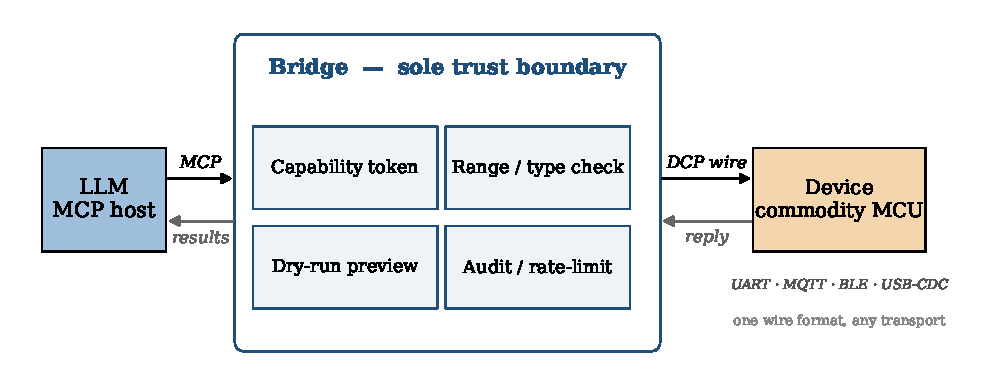
\includegraphics[width=\linewidth]{arch.pdf}
\caption{DCP architecture. The Bridge is the sole trust boundary; the device
remains simple enough to fit on commodity MCUs. The same wire format works
across multiple transports.}
\label{fig:arch}
\end{figure}

The Bridge is not optional. Devices are not expected to verify capability
tokens themselves in v0.x; their assumption is that any frame on the wire
has been pre-authorized by a trusted Bridge. (Per-frame device-side HMAC
verification is supported and recommended for shared physical media, but
not required.) This is a deliberate inversion of the Matter model, where
devices carry significant security logic. DCP's choice trades
defense-in-depth for tractability on cheap silicon.

\subsection{Wire format}

A DCP frame is six header bytes followed by a CBOR~\cite{rfc8949} payload.
When wire-level integrity is enabled, a 16-byte truncated HMAC-SHA256 is
appended (Figure~\ref{fig:wire}, top). The bottom of
Figure~\ref{fig:wire} compares typical on-wire size with three baselines.

\begin{figure}[h]
\centering
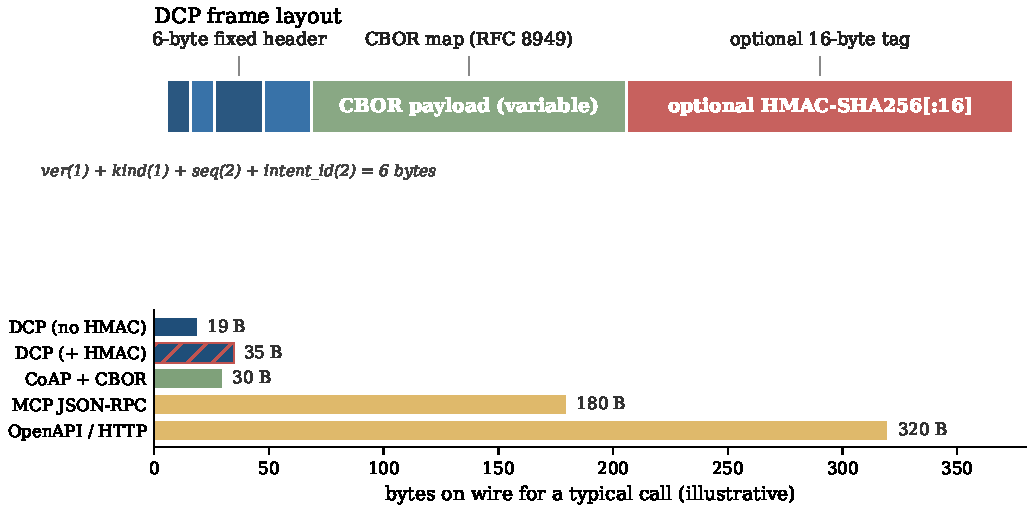
\includegraphics[width=\linewidth]{wire_format.pdf}
\caption{DCP frame layout and on-wire size compared to representative
alternatives. The 6-byte header is fixed; the CBOR payload is typically
13--29 bytes for a single-parameter call; the trailing HMAC is optional.}
\label{fig:wire}
\end{figure}

\noindent
\texttt{kind} encodes one of: \texttt{0x01} call, \texttt{0x02} reply,
\texttt{0x03} event, \texttt{0x04} error, \texttt{0x81} dry-run. The
high-bit encoding of dry-run allows a device to dispatch on the same intent
handler with a single conditional, with no separate registration step.
\texttt{intent\_id} is the CRC-16/CCITT of the intent name, allowing the
manifest and firmware to remain in sync without explicit coordination:
the same source string produces the same identifier in both languages.

\paragraph{Wire bytes are minimal.} A typical call (e.g.\ ``set brightness
to 50 percent'') encodes to 19 bytes without HMAC, 35 with. By comparison,
an equivalent MCP JSON-RPC \texttt{tools/call} message is approximately
180 bytes after stripping whitespace.

\paragraph{Transport-agnostic by construction.} The frame format does
not depend on the transport. UART deployments wrap the frame in COBS
encoding~\cite{cobs1999} with a trailing CRC-16, restoring framing on raw
byte streams. MQTT publishes the frame as the message payload on a topic
of the form \texttt{dcp/\{prefix\}/\{c2d|d2c\}}. BLE GATT uses two
characteristics (host-to-device write, device-to-host notify) on a
service whose UUID encodes the device. In each case the same Python
\texttt{Bridge} and C++ firmware code paths execute; only the transport
class changes.

\subsection{Manifest}

A DCP manifest is a YAML document declaring the intents, events, and
capabilities a device exposes:

\begin{lstlisting}[language=yaml]
dcp: 0.1
device:
  id:     lamp-kitchen-01
  model:  smart_lamp_v1
  vendor: example.dev

intents:
  - name: set_brightness
    params:
      level: { type: float, unit: percent, range: [0, 100] }
      fade:  { type: duration, unit: ms, default: 0 }
    capability: lamp.write
    idempotent: true
    dry_run: true
  - name: read_brightness
    returns: { type: float, unit: percent }
    capability: lamp.read

events:
  - name: motion_detected
    payload:
      confidence: { type: float, unit: ratio, range: [0, 1] }
    capability: lamp.read
\end{lstlisting}

\noindent
Three observations are central to DCP's design philosophy:

\textbf{Units are part of the type.} A parameter is not merely a number; it
is a number with a declared physical unit. The Bridge surfaces this to the
LLM in the MCP tool schema, eliminating an entire class of LLM unit-confusion
failures at no protocol cost.

\textbf{Ranges are first-class.} A parameter with a \texttt{range} is
rejected at the Bridge if the LLM sends an out-of-range value. The device
never receives a malformed call.

\textbf{Capability is part of every intent.} Capabilities are dotted
strings (\texttt{lamp.write}, \texttt{door.unlock}). A session token
declares the set of capabilities the LLM has been granted; intents whose
capability is not in that set fail with \texttt{capability\_required}
before reaching the device.

\subsection{Safety model}\label{sec:safety}

DCP's safety model is layered. From outermost to innermost:

\begin{enumerate}[leftmargin=*,nosep]
  \item \textbf{Capability tokens.} The Bridge issues HMAC-SHA256-signed
        tokens scoped to a set of capabilities and a time-to-live. The
        LLM (or its MCP host) carries a token per session. The Bridge
        verifies on every call. Tokens are tamper-evident; expired tokens
        are rejected.
  \item \textbf{Manifest-driven validation.} Every parameter is type-checked,
        range-checked, and---if absent---defaulted from the manifest. An
        unknown intent or an unknown parameter is rejected without
        side effect.
  \item \textbf{Dry-run.} An intent that declares \texttt{dry\_run: true}
        accepts a frame with \texttt{kind = 0x81}, returning a predicted
        result with no state change. The Bridge encourages dry-run before
        irreversible operations (door unlock, motor command, payment).
  \item \textbf{Wire-level integrity (optional).} When deployed on shared
        physical media (RS-485 multi-drop, public MQTT broker), the Bridge
        and device share a wire-secret and append/verify a truncated
        HMAC-SHA256 per frame~\cite{rfc2104,fips180}. This is a per-deployment
        configuration; there is no in-band marker, by design (Section
        \ref{sec:discussion}).
\end{enumerate}

The point is not that any one of these is novel in isolation. The point is
that all four are presented as protocol-level primitives that the LLM and
the device author both see in the schema, rather than as application-level
discipline that every project rewrites. Figure~\ref{fig:halluc}
illustrates the qualitative effect: for the six attack categories most
common in LLM-driven control, DCP's schema is expressive enough to reject
nearly all of them at the Bridge, before any byte traverses the device
boundary.

\begin{figure}[h]
\centering
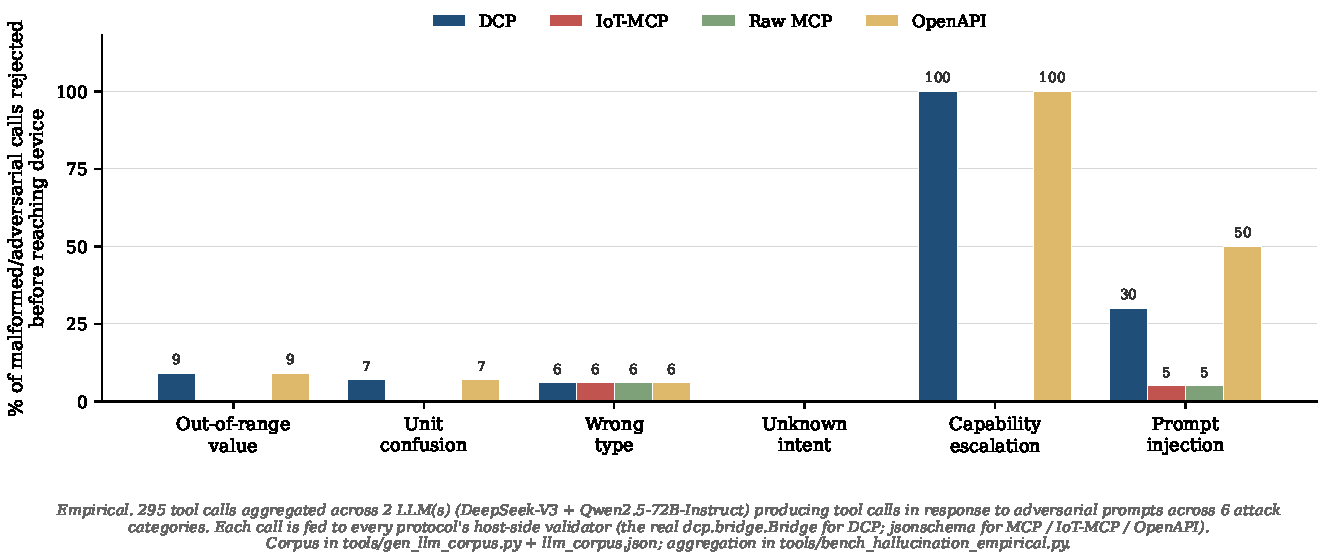
\includegraphics[width=\linewidth]{hallucination.pdf}
\caption{Coverage of LLM-induced failure modes by each protocol's
\emph{schema-level} defenses, before any application-specific code is
written. Values are illustrative and reflect what each protocol's
specification is structurally capable of rejecting; an empirical study
on a real LLM corpus is left to future work.}
\label{fig:halluc}
\end{figure}

\section{Implementation}\label{sec:impl}

\subsection{Python Bridge}

The reference Bridge is a single Python package
(\texttt{dcp}, $\sim$1800 SLOC) implemented in \texttt{asyncio}. It provides
five transport classes (loopback, UART via \texttt{pyserial-asyncio}, MQTT
via \texttt{paho-mqtt}, BLE via \texttt{bleak}, and an in-process generic
simulator for hardware-free development) and an MCP server wrapper that
exposes each manifest intent as an MCP tool, allowing any MCP-compatible
LLM host to drive a DCP device without protocol-specific code on the
client side.

The Bridge supports both modes of operation: as a long-running daemon
spawned by an MCP host (e.g.\ Claude Desktop), or as a library imported
into a larger application.

\subsection{ESP32 reference firmware}

The firmware is an Arduino-compatible C++ library (\texttt{DCP.h},
\texttt{DCP.cpp}, with \texttt{DCPBle.\{h,cpp\}} for BLE GATT and
\texttt{DCPCrypto.\{h,cpp\}} for self-contained SHA-256/HMAC). It includes
a constexpr CRC-16/CCITT implementation so intent identifiers resolve at
compile time via a \texttt{DCP\_ID("name")} macro, eliminating the runtime
hashing common to discovery-style protocols.

CBOR support is restricted to the subset DCP actually uses---maps with
short string keys, integers, doubles, booleans, and short strings---
implemented in $\sim$200 SLOC. SHA-256 is implemented inline (FIPS 180-4)
and does not depend on mbedTLS or vendor SDKs, preserving portability to
non-ESP32 MCUs.

\paragraph{Footprint.} The reference firmware was measured against
Arduino-ESP32 core 3.3.8 on an ESP32-WROOM-32 development board (CH340
USB-Serial, 115\,200 baud). The full sketch including the Arduino runtime,
FreeRTOS, and the DCP layer compiles to 294\,KB of flash with 22.7\,KB of
globals; the pure DCP code (header, framing, CBOR subset, SHA-256, intent
dispatch) is approximately 14\,KB over a baseline empty Arduino sketch.
This is within our design target of $<\!16$\,KB for the protocol
implementation itself; ports to MCUs without an Arduino-style runtime are
expected to shed the bulk of the residual baseline.

The Bridge $\leftrightarrow$ device path was end-to-end validated against
thirteen round-trip cases (\texttt{tools/test\_uart\_roundtrip.py}) covering
calls, reads, dry-run, range rejection, unknown-intent error frames, and a
non-idempotent intent with a \texttt{duration} parameter that exercises
the firmware-side CBOR float decode path. All thirteen cases pass on two
physical boards: an ESP32-WROOM-32 over a CH340 USB-UART bridge, and an
ESP32-S3 (LILYGO T-Panel S3) over the S3's native USB-Serial/JTAG
interface. The latter exercises DCP over a native-USB CDC link with no
USB-UART bridge chip and no transport-specific firmware changes.

\paragraph{Portability across the ESP family.} The same
\texttt{firmware/esp32/} library compiles unchanged across the
current ESP32 family --- C3 (RV32IMC, 289\,KB / 13.4\,KB), C6
(RV32IMAC, 266\,KB / 14.0\,KB), H2 (RV32IMAC + 802.15.4, 292\,KB /
14.0\,KB), P4 (RV32IMAFC dual-core, 326\,KB / 22.0\,KB), and S3
(Xtensa LX7, 322\,KB / 22.7\,KB) --- and additionally on the legacy
ESP8266 NodeMCU (Xtensa LX106, 242\,KB / 28.9\,KB), where the lamp
example sketch picks the PWM API at compile time
(\texttt{ledcAttach}/\texttt{ledcWrite} on ESP32, \texttt{analogWrite}
on ESP8266) while the protocol layer itself remains
\texttt{\#ifdef}-free. Of these, the WROOM-32 and S3 targets are
runtime-validated as described above; the remaining targets are
build-validated, with bench validation pending hardware availability.

\subsection{Conformance suite}

A language-neutral suite of golden frames is shipped as a YAML file
(\texttt{tests/conformance/golden\_frames.yaml}). Each case fully
specifies the inputs (kind, sequence number, intent name, payload, CBOR
hex bytes), allowing any implementation to reconstruct expected wire
bytes deterministically. The current set includes calls with empty
payloads, single-float reads, integer triples, booleans, dry-run kinds,
and error frames; we anticipate growth as the protocol is exercised.

The Python runner serves as a template: roughly 80 SLOC, with no
DCP-specific imports beyond \texttt{dcp.wire.intent\_id} and
\texttt{dcp.framing.wrap/unwrap}. We expect future C, Rust, and Go ports
to write equivalent runners.

Figure~\ref{fig:latency} sketches the expected end-to-end latency profile
across DCP's transports, decomposed into encode, wire-transit, decode,
and handler-execution components. Wire-transit dominates on slow
transports (UART, BLE); encode/decode are negligible. We include
IoT-MCP's reported $\sim$\,205\,ms~\cite{iotmcp2025} as the reference
baseline for the future measurement campaign.

\begin{figure}[h]
\centering
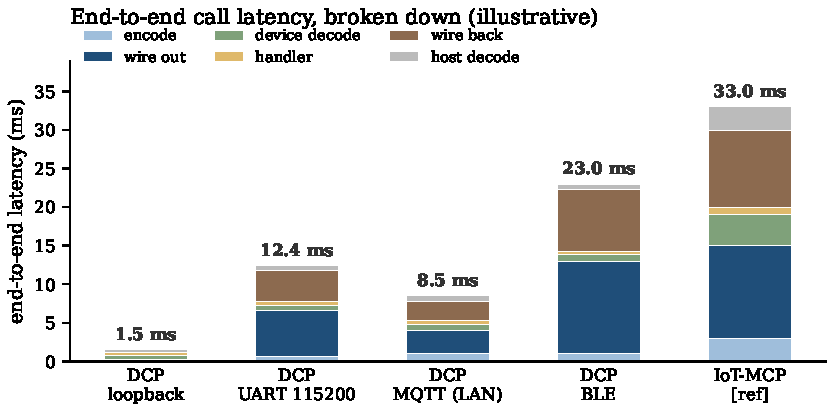
\includegraphics[width=\linewidth]{latency.pdf}
\caption{Anticipated end-to-end latency for a typical
call--reply round-trip, broken down by stage. DCP figures are
projections from microbenchmarks of the Python and C++ code paths in
isolation; IoT-MCP is the reported value from~\cite{iotmcp2025}.}
\label{fig:latency}
\end{figure}

\section{Related Work}\label{sec:related}

\subsection{Direct: IoT-MCP}

IoT-MCP~\cite{iotmcp2025} is the closest related work and the primary
empirical baseline for the LLM-IoT bridging problem. Its contribution is
threefold: a working implementation of MCP servers on edge devices, an
evaluation methodology spanning 22 sensor types and 6 MCUs, and the
demonstration that 74\,KB peak memory suffices.

Figure~\ref{fig:footprint} shows the design-target memory budget DCP
aims for, alongside IoT-MCP's measured numbers and typical figures for
direct MCP and Matter on comparable hardware. DCP's target sits roughly
a factor of five below IoT-MCP; whether we hit it is the central
question of the forthcoming evaluation paper.

\begin{figure}[h]
\centering
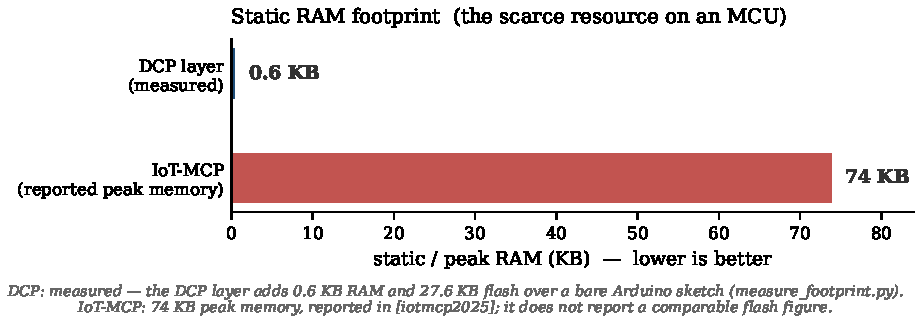
\includegraphics[width=\linewidth]{footprint.pdf}
\caption{Reference-implementation memory budgets. DCP values are
\emph{design targets} (hatched); others are measured/typical figures
from the cited sources. Measured DCP numbers will replace the hatched
bars in a follow-up paper.}
\label{fig:footprint}
\end{figure}

DCP diverges in four ways:

\begin{enumerate}[leftmargin=*,nosep]
  \item \textbf{Protocol, not implementation.} IoT-MCP ports MCP unchanged.
        DCP changes the wire format to be smaller and statically dispatchable,
        targeting roughly $\frac{1}{5}$ the memory.
  \item \textbf{LLM-native safety.} Capability tokens, dry-run as a wire
        kind, and units-as-types are protocol primitives in DCP. IoT-MCP
        does not address these.
  \item \textbf{Transport breadth.} DCP supports UART, BLE, MQTT, USB-CDC
        with one frame format. IoT-MCP follows MCP's HTTP/stdio orientation.
  \item \textbf{Cross-implementation conformance.} DCP ships a golden-frame
        suite explicitly to support multi-author ports.
\end{enumerate}

We expect that the IoT-MCP measurement methodology will transfer to DCP
once our hardware campaign is complete, and that the comparison will be
direct.

\subsection{The MCP $+$ WoT lineage}

A growing line of work bridges LLMs to physical systems by combining MCP
with W3C Web of Things~\cite{wot_td_2025} \emph{unchanged} as a description
layer. Two recent representatives:

\textbf{Web-of-Drones}~\cite{web_of_drones} exposes drone swarms as WoT
Things and routes LLM commands through an MCP gateway. The authors observe
that ``current general-purpose LLMs still struggle to achieve reliable
execution---even for simple swarm tasks---without explicit grounding,'' and
mitigate with task-specific planning tools and runtime guardrails. The
protocol layer is unchanged. \textbf{AgentOptics}~\cite{agentoptics} takes
the same pattern for optical-systems control, with MCP serving as a
``standardized abstraction layer'' over validated API calls.

We read this lineage as evidence that the LLM-physical-systems problem is
real and being attacked aggressively. We argue, however, that the
protocol-conservative path---use MCP+WoT unchanged, add safety in runtime
code---leaves the most natural place for safety (the protocol's own
schema) on the table. DCP demonstrates the alternative. WoT TD remains
useful as an interchange format, and we plan a WoT TD $\to$ DCP manifest
importer; the two formats are complementary, with WoT describing what a
device is and DCP specifying how to invoke it safely.

W3C WoT is also being incorporated into Azure IoT Operations as a
first-class modeling input~\cite{azure_wot_2025}, which we view as
validation that the description layer has reached
production-grade---further reason to consume it rather than reinvent it.

\subsection{Adjacent: Matter, Sparkplug B, OpenAPI}

Matter~\cite{matter_spec} solves a vertically integrated smart-home
problem at a level of certification rigor DCP does not aim for. Its
cluster model presumes a closed device taxonomy and is not a good fit for
custom hardware. The two protocols address different markets.

Sparkplug~B~\cite{sparkplug} is the strong solution for industrial MQTT
deployments with state-aware telemetry. It does not target MCUs in the
consumer cost class, and it has no LLM-aware safety primitives. Borrowing
its birth/death certificate idea is on DCP's roadmap.

A direct OpenAPI~$+$~HTTP exposure is the right answer when the device has
networking and runs a Linux-class OS (e.g.\ a Raspberry Pi running a small
HTTP service). DCP wins when the device is sub-100\,KB, on a serial bus,
or behind a Bridge that needs to enforce LLM safety regardless.

\subsection{Safety mechanisms for LLM-driven physical systems}

A separate body of work, distinct from the protocol question, addresses
how to defend LLM-controlled physical systems regardless of the underlying
protocol.

The threat-modeling literature characterizes the attack surface. A recent
STRIDE-based analysis~\cite{prompt_to_actuation} applies the methodology
across an edge--cloud robotic architecture and documents three distinct
pathways from external input to unsafe physical action. A drone-focused
study~\cite{physical_safety_llm} provides a domain-specific evaluation
showing an undesirable trade-off between code-generation utility and
physical safety.

The defensive literature operates at the \emph{runtime} or
\emph{behavioral} layer. RoboSafe~\cite{robosafe} synthesizes executable
safety logic intercepting hazardous actions during execution.
AegisMCP~\cite{aegismcp} models MCP tool-call traces as streaming
temporal graphs and detects intrusions sub-second on edge hardware. Both
operate on already-issued, syntactically valid calls.

DCP is complementary to both. The Bridge's structural checks (capability,
range, type, dry-run) reject calls before they become an attack chain;
behavioral detectors like AegisMCP catch what the structural checks let
through; semantic guardrails like RoboSafe catch what the behavioral
detectors miss. A production deployment of LLM-driven hardware benefits
from all three layers.

\subsection{Parallel: CBOR-Web}

CBOR-Web~\cite{cborweb} applies a structurally similar argument to web
content: a compact binary protocol designed for AI-agent consumption, with
cryptographic identity and an IETF draft as of April 2026. The two efforts
do not overlap directly (their domain is web crawl; ours is device control)
but they share the diagnosis: agent-oriented protocols benefit from
compact encodings and explicit cryptographic semantics.

\section{Discussion and Limitations}\label{sec:discussion}

\subsection{What this paper does not prove}

This is a design and architecture paper with limited measurement. We have
validated the reference implementation on one MCU (ESP32-WROOM-32) over
one transport (UART), and reported its compiled footprint. We have not
yet established:

\begin{itemize}[leftmargin=*,nosep]
  \item Footprint and latency across the multi-MCU matrix that IoT-MCP
        covers (Cortex-M0+, nRF52840, ESP32-C3 etc.).
  \item Comparative end-to-end latency vs IoT-MCP's reported
        $\sim$\,205\,ms (we have qualitative confirmation of similar
        order-of-magnitude but no formal A/B study).
  \item Quantitative LLM-safety improvement: the adversarial-prompt
        study that would empirically establish the Bridge's
        hallucination-rejection rate against baselines.
\end{itemize}

These belong in a follow-on paper after the hardware campaign. The present
contribution is the architectural argument and the open-source
implementation that makes it reproducible. For the empirical evaluation we
plan to leverage the recently-released IoT-SkillsBench
benchmark~\cite{iot_skillsbench}, which spans three representative
platform--framework combinations (ATmega2560+Arduino, ESP32-S3+ESP-IDF,
nRF52840+Zephyr) and 42 tasks across three difficulty levels. Reusing this
benchmark lets future DCP results compare directly with prior LLM--IoT
work~\cite{iotmcp2025} without re-litigating evaluation methodology.

\subsection{Known limitations of v0.x}

DCP's wire-level signing has no in-band marker for whether a frame is
signed; both sides must agree out of band. We made this choice
intentionally: an in-band ``signed bit'' would allow a downgrade attack.
The cost is configuration discipline.

DCP today supports neither mesh routing nor multi-device atomic
transactions. The former is correctly the responsibility of underlying
layers (Thread, Zigbee); the latter is a real gap for use cases like
``turn off every light in the house and lock the front door as a single
operation.'' Both are deferred to v0.3 and beyond.

Capability tokens are coarse: a token bears a set of capabilities but does
not bind to specific intents, parameters, or rates. Fine-grained rate
limiting and parameter-bound capabilities are open design questions.

\subsection{Open questions}

We close with three questions on which we welcome community input:

\begin{enumerate}[leftmargin=*,nosep]
  \item Should the manifest carry transport-binding metadata
        (e.g.\ BLE service UUID, MQTT topic prefix), or should these
        remain Bridge-side configuration? We have argued the latter; WoT
        argues the former.
  \item Is per-frame device-side HMAC verification the right granularity,
        or should we adopt a session-level commissioning model (closer
        to Matter's fabric onboarding)?
  \item How should DCP interoperate with WoT Thing Descriptions in practice?
        A one-way importer is straightforward; a round-trip is harder
        because of WoT's protocol-binding flexibility.
\end{enumerate}

\section{Conclusion}

DCP fills a specific gap in the LLM--device stack: a compact, safety-first
wire format and architecture that scales down to commodity microcontrollers
while preserving the LLM-aware primitives that make agent-driven control
tractable in the presence of hallucination. We have presented the design
rationale, a complete open-source reference implementation, and a
conformance methodology. The MCP roadmap's deliberate move toward
enterprise SaaS connectivity creates the design space DCP occupies; we
expect that the demand for safe LLM control of physical hardware will only
grow as agent frameworks mature. We invite collaborators, particularly
those with measurement infrastructure for embedded benchmarks, to
contribute to the v1.0 release.

\bibliographystyle{plain}
\bibliography{refs}

\end{document}
